\documentclass{article}
\usepackage[utf8]{inputenc}

\usepackage[paperwidth=8.5in, paperheight=11in, top=1in, bottom=.5in, left=.5in, right=.5in]{geometry}
\usepackage{fancyhdr, graphicx,tikz,amsmath,multicol,paracol,pgfplots}
\usepackage[inline]{enumitem}

\pagestyle{fancy}
\lhead{\large{\textbf{Module 7: Periodic Functions (PF) - Readiness Assurance Test}}}
\chead{}
\rhead{}
\lfoot{}
\cfoot{}
%\rfoot{\thepage/\pageref{LastPage} }
\setlength{\headheight}{14pt} %added in bc warning

%%% LIST ANSWER KEY HERE

% 1 B
% 2 D
% 3 A
% 4 B
% 5 D
% 6 A
% 7 B
% 8 C
% 9 D
% 10 B


\begin{document}


\begin{enumerate}

% Determine the equation from a table.

\item Which of the following equations are satisfied by the points in the table below?

    \begin{center}
    \begin{tabular}{ |c|c| } 
        \hline
        $x$ & $y$ \\
        \hline
        $-4$ & $-21$ \\ 
        $-1$ & $-6$ \\ 
        $2$ & $9$ \\
        $5$ & $24$ \\
        $8$ & $39$ \\
        \hline
    \end{tabular}
    \end{center}
\vspace{5pt}

  \begin{enumerate}
  \begin{multicols}{4}
  \item $y=3x-21$  
  \item $y=5x-1$ %correct 
  \item $y=15x-21$
  \item $y=x-17$
  \end{multicols}
  \end{enumerate}

\vspace{5pt}
\hspace{-15pt}\textbf{For questions 2-4, use the unit circle to determine the exact values.}

% Determine exact value of trigonometric functions using the unit circle.

\item $\sin\left(270^{\circ}\right)$

        \begin{enumerate}
        \begin{multicols}{4}
          
          \item $0$ 
          \item $\frac{1}{2}$ 
          \item undefined
          \item $-1$ %correct
        \end{multicols}
        \end{enumerate}

\item $\cos\left(\dfrac{2\pi}{3}\right)$

        \begin{enumerate}
        \begin{multicols}{4}
          
          \item $-\frac{1}{2}$ %correct
          \item $\frac{\sqrt{3}}{2}$ 
          \item undefined
          \item $-\frac{\sqrt{3}}{2}$
        \end{multicols}
        \end{enumerate}

\item $\csc\left(\dfrac{4\pi}{3}\right)$

        \begin{enumerate}
        \begin{multicols}{4}
          
          \item $-\sqrt{3}$ 
          \item $-\frac{2\sqrt{3}}{3}$ %correct
          \item $-\frac{1}{2}$
          \item $-\sqrt{2}$
        \end{multicols}
        \end{enumerate}

% Find the domain and range of a function from its graph.
\vspace{5pt}
\hspace{-10pt}\textbf{The function $f(x)$ is pictured below. Use this graph for questions 5-6.}

        \begin{center}
        \item 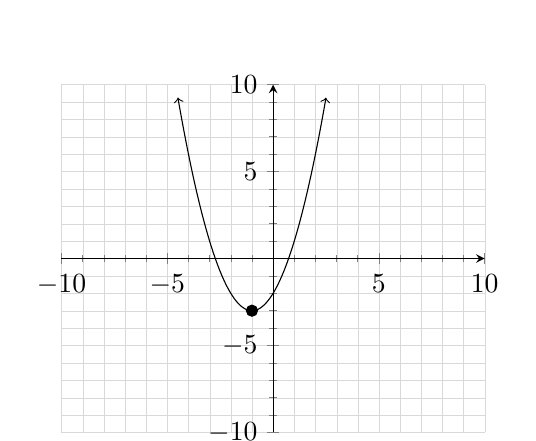
\begin{tikzpicture}   
        \begin{axis}[
                height=6cm,
                axis lines=center,
                grid=both,
                grid style={line width=.05pt, draw=gray!30},
                minor tick num=4,
                xtick={-10,-5,...,10},
                ytick={-10,-5,...,10},
                xmin=-10, xmax=10,
                ymin=-10, ymax=10,
                ]
                \addplot [
                    domain=-4.5:2.5, 
                    samples=200, 
                    color=black,
                    <->,
                    ]{(x+1)^2-3};
                \addplot[mark=*] coordinates {(-1,-3)};
        \end{axis}
        \end{tikzpicture}              
        \end{center}

\item Find the domain of $f(x)$.        

        \begin{enumerate}
        \begin{multicols}{4}
              \item $[-3, \infty)$ 
              \item $(-1, -3)$
              \item $(-1, \infty)$
              \item $(-\infty,\infty)$ %correct 
        \end{multicols}
        \end{enumerate}  

\item Find the range of $f(x)$.      

        \begin{enumerate}
        \begin{multicols}{4}
              \item $[-3, \infty)$ %correct
              \item $(-1, -3)$
              \item $(-1, \infty)$
              \item $(-\infty,\infty)$   
              
        \end{multicols}
        \end{enumerate}
\pagebreak

%Determine angle from unit circle.
\item What angle measure on the unit circle gives a $y$-value of $-\frac{\sqrt{3}}{2}$?

\begin{enumerate}
 \begin{multicols}{4}
          \item $210^{\circ}$ 
          \item $\frac{4\pi}{3}$ %correct
          \item $60^{\circ}$ 
          \item $\frac{\pi}{6}$
        \end{multicols}
        \end{enumerate}

%Determine graph from table.

\item Which graph matches the table given below?

\begin{center}
\begin{tabular}{ |c|c| } 
\hline
$x$ & $f(x)$ \\
\hline
$-2$ & $1$ \\ 
$1$ & $2$ \\ 
$5$ & $-3$ \\
$-3$ & $5$ \\
\hline
\end{tabular}
\end{center}
\vspace{5pt}

        \begin{enumerate}
  \begin{multicols}{2}
        \item 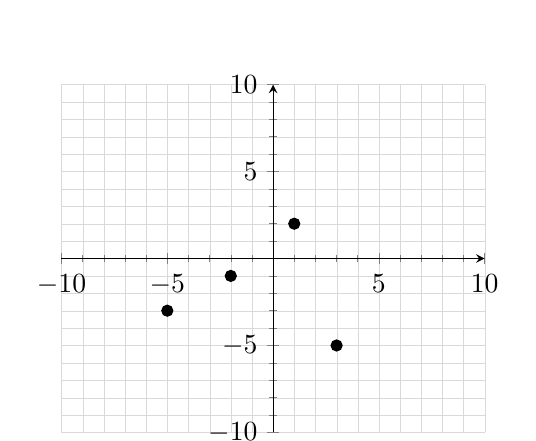
\begin{tikzpicture}   
        \begin{axis}[
                height=6cm,
                axis lines=center,
                grid=both,
                grid style={line width=.05pt, draw=gray!30},
                minor tick num=4,
                xtick={-10,-5,...,10},
                ytick={-10,-5,...,10},
                xmin=-10, xmax=10,
                ymin=-10, ymax=10,
                ]
                \addplot[mark=*] coordinates {(-2,-1)};
                \addplot[mark=*] coordinates {(1,2)};
                \addplot[mark=*] coordinates {(-5,-3)};
                \addplot[mark=*] coordinates {(3,-5)};
        \end{axis}
        \end{tikzpicture}

        \item 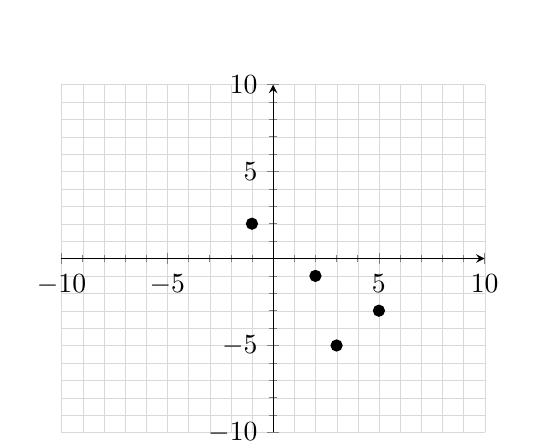
\begin{tikzpicture}
        \begin{axis}[
                height=6cm,
                axis lines=center,
                grid=both,
                grid style={line width=.05pt, draw=gray!30},
                minor tick num=4,
                xtick={-10,-5,...,10},
                ytick={-10,-5,...,10},
                xmin=-10, xmax=10,
                ymin=-10, ymax=10,
                ]
                \addplot[mark=*] coordinates {(2,-1)};
                \addplot[mark=*] coordinates {(-1,2)};
                \addplot[mark=*] coordinates {(5,-3)};
                \addplot[mark=*] coordinates {(3,-5)};
        \end{axis}
        \end{tikzpicture}

        \item 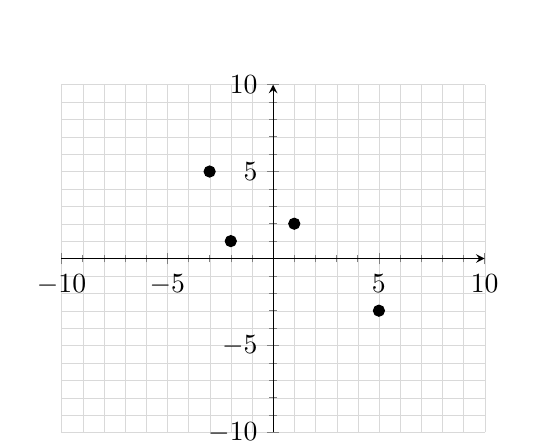
\begin{tikzpicture}   %correct
        \begin{axis}[
                height=6cm,
                axis lines=center,
                grid=both,
                grid style={line width=.05pt, draw=gray!30},
                minor tick num=4,
                xtick={-10,-5,...,10},
                ytick={-10,-5,...,10},
                xmin=-10, xmax=10,
                ymin=-10, ymax=10,
                ]
                \addplot[mark=*] coordinates {(-2,1)};
                \addplot[mark=*] coordinates {(1,2)};
                \addplot[mark=*] coordinates {(5,-3)};
                \addplot[mark=*] coordinates {(-3,5)};
        \end{axis}
        \end{tikzpicture}

        \item 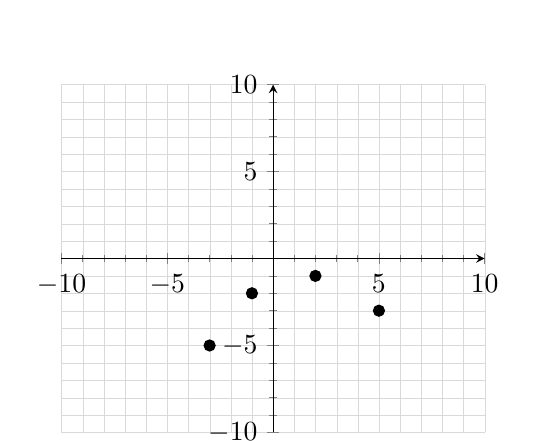
\begin{tikzpicture}   
        \begin{axis}[
                height=6cm,
                axis lines=center,
                grid=both,
                grid style={line width=.05pt, draw=gray!30},
                minor tick num=4,
                xtick={-10,-5,...,10},
                ytick={-10,-5,...,10},
                xmin=-10, xmax=10,
                ymin=-10, ymax=10,
                ]
                \addplot[mark=*] coordinates {(2,-1)};
                \addplot[mark=*] coordinates {(-1,-2)};
                \addplot[mark=*] coordinates {(5,-3)};
                \addplot[mark=*] coordinates {(-3,-5)};
        \end{axis}
        \end{tikzpicture}
    
      
  \end{multicols}
  
  \end{enumerate}

%Determine the equation given transformations.
\item The function $y=f(x)$ undergoes two translations: $5$ units right and $2$ units down. What is the new equation for the translated function?

 \begin{enumerate}
 \begin{multicols}{4}
          \item $y+2=f(x+5)$ 
          \item $y+2=f(x-5)$
          \item $y-2=f(x+5)$
          \item $y-2=f(x-5)$ %correct
        \end{multicols}
        \end{enumerate}
        
%Determine transformation from the equation.
\item The graph of $y+5=-2f(3(x-3))$ is the image of the graph $y=f(x)$ after a combination of transformations. Which statement below is true?

 \begin{enumerate}
          \item The graph $y=f(x)$ was translated $3$ units down.
          \item The graph $y=f(x)$ was compressed horizontally by a factor of $\frac{1}{3}$. %correct
          \item The graph $y=f(x)$ was stretched horizontally by a factor of $2$.
          \item The graph $y=f(x)$ was reflected across the $y$-axis. 
        \end{enumerate}
        
\end{enumerate}


\end{document}